\documentclass[12.5pt]{scrartcl}

%\usepackage[romanian, english, ngerman]{babel}
\usepackage[T1]{fontenc}
\usepackage{lmodern}
\usepackage{amsmath}
\usepackage{amsfonts}
\usepackage{amssymb}
\usepackage{mathrsfs}
\usepackage{microtype}
\usepackage[utf8x]{inputenc}
\usepackage{graphicx}
\usepackage{setspace}
\usepackage{float}

%\linespread{1.5}
\usepackage{multirow}
\usepackage{tabularx}


\title{RoboFace}
\date{\vspace{-7ex}}
\begin{document} 
	\maketitle
	\thispagestyle{empty}
	
	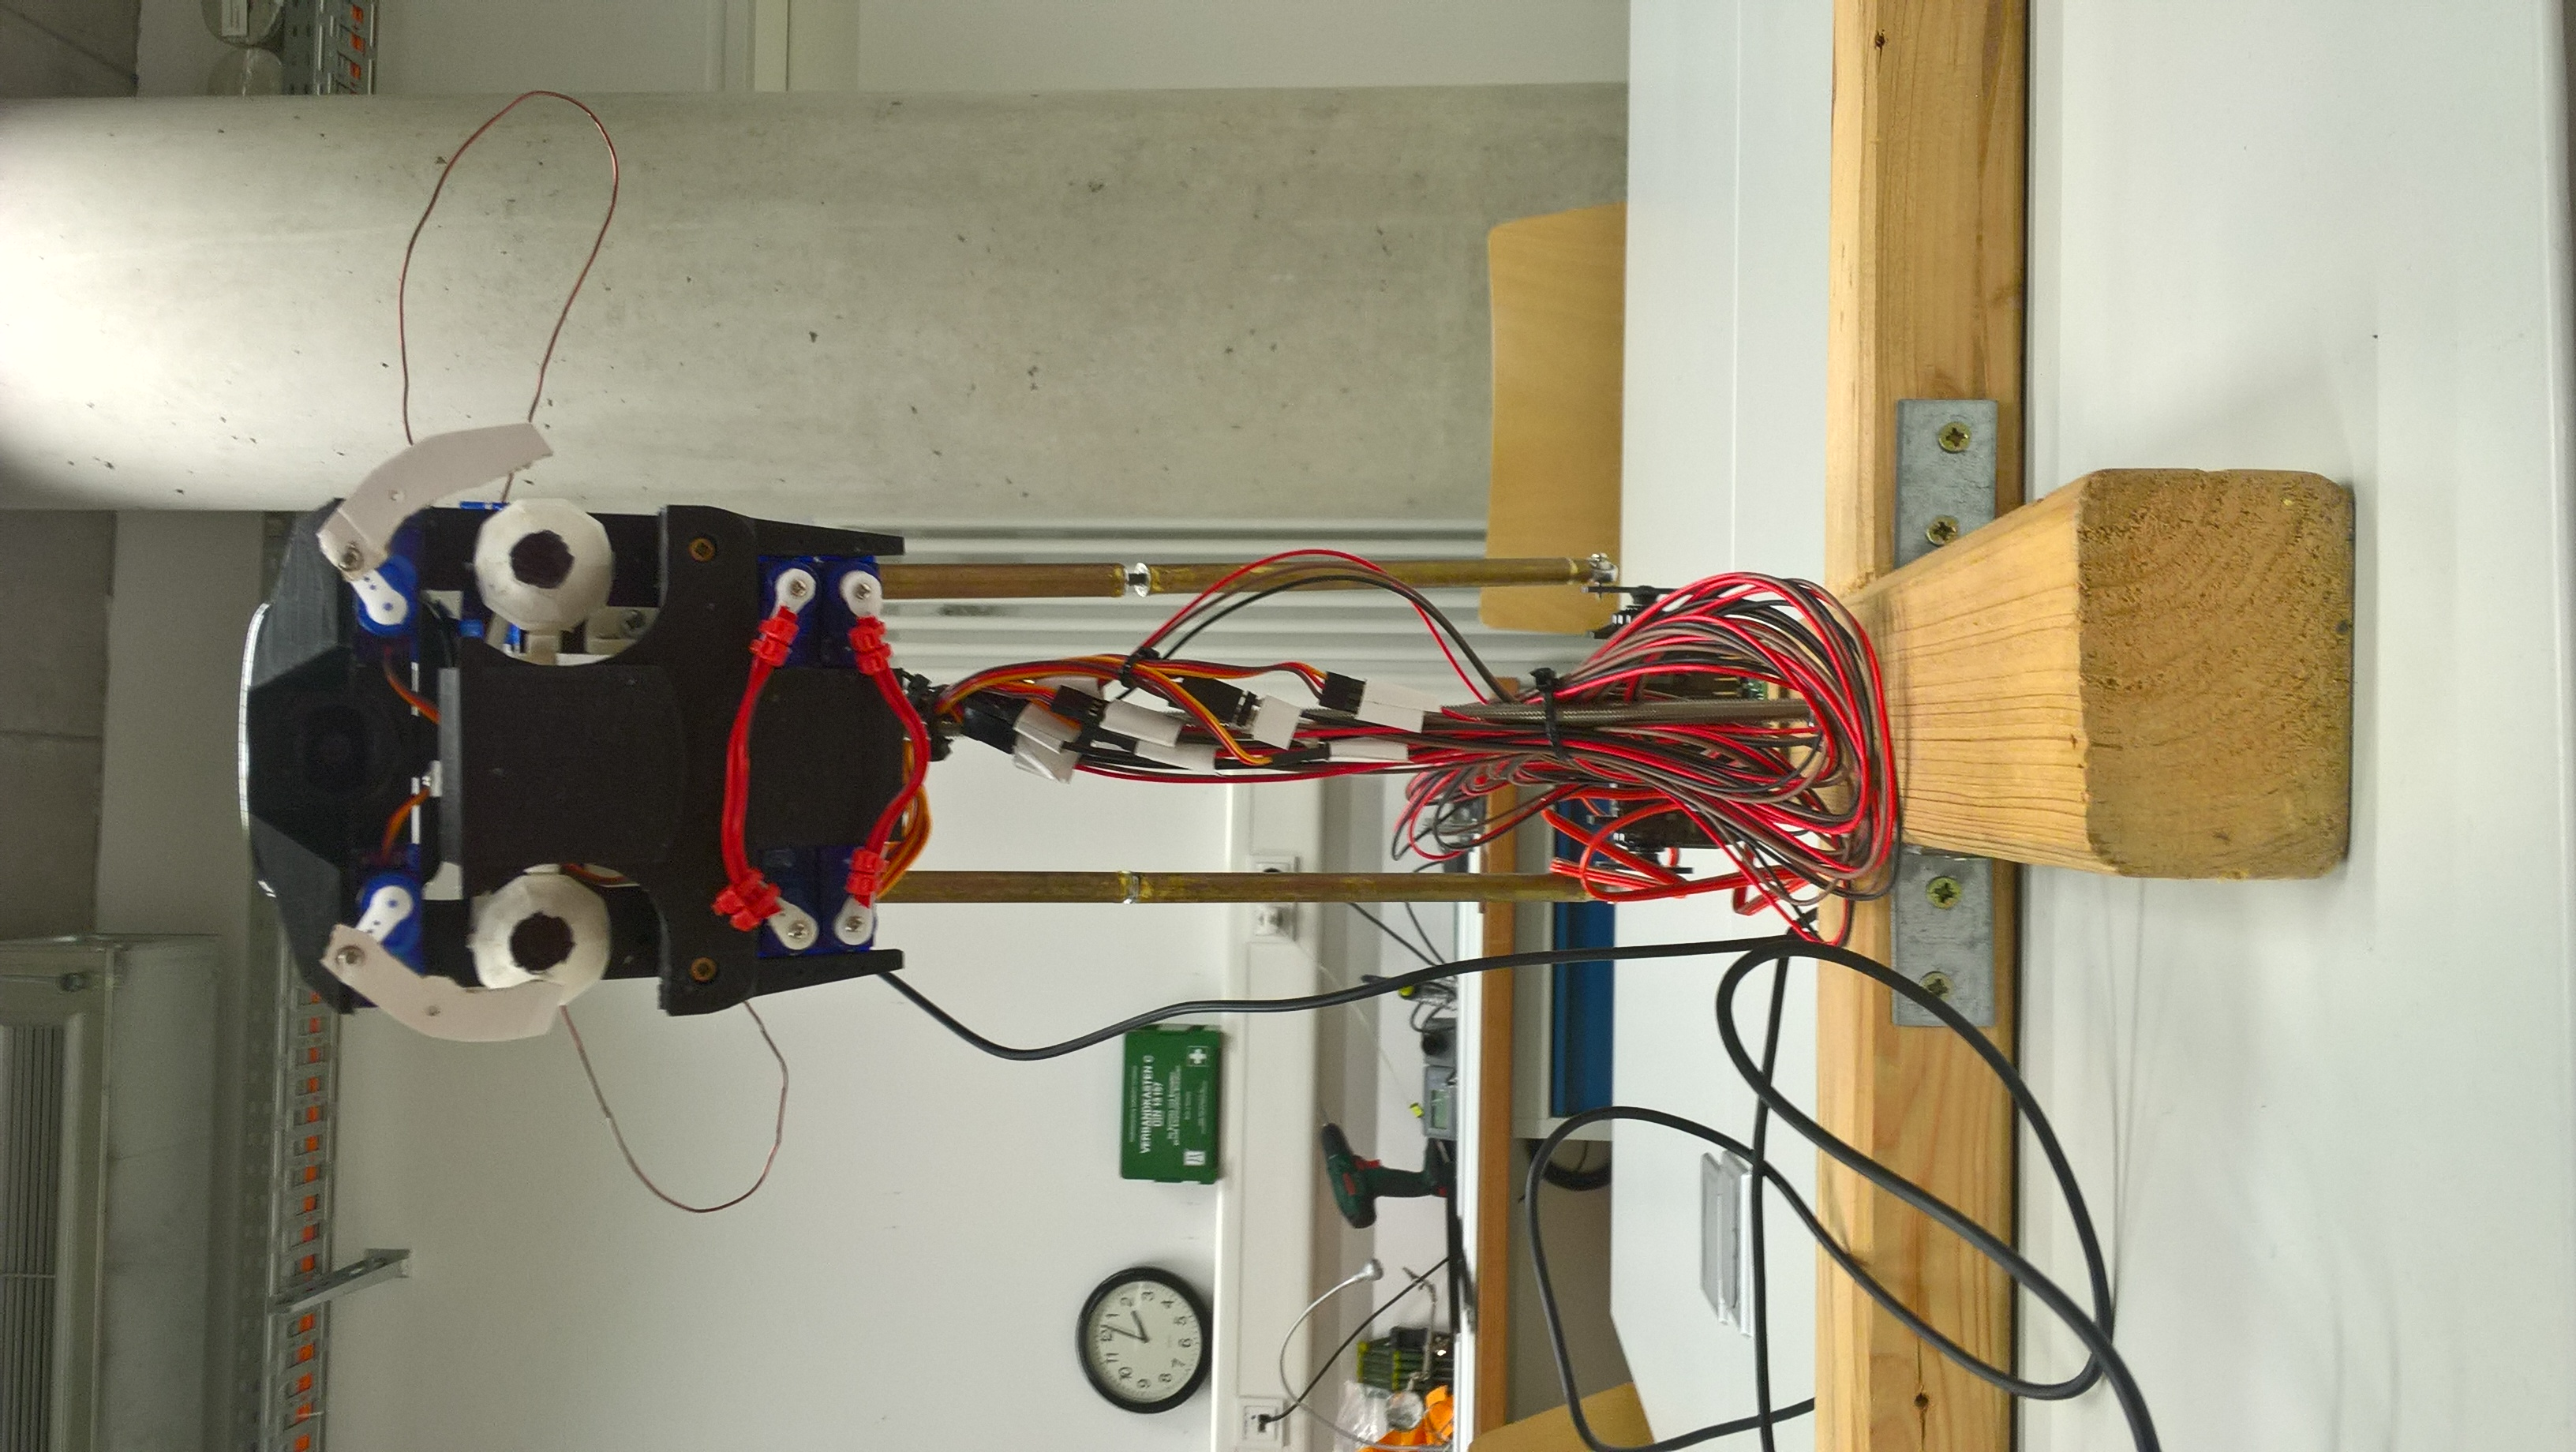
\includegraphics[width=0.88\linewidth]{images/roboFace}
	
	\begin{tabularx}{\textwidth}{Xl} 
		Kevin Kiefer      & Letitia Parcalabescu \\ 
		5\textsuperscript{th} semester informatics  & 3\textsuperscript{rd} semester informatics \\ 
	\end{tabularx}
	
	Supervisors: Gero Plettenberg and Benjamin Reh
	
	\vspace*{8mm}
	\begin{center}
		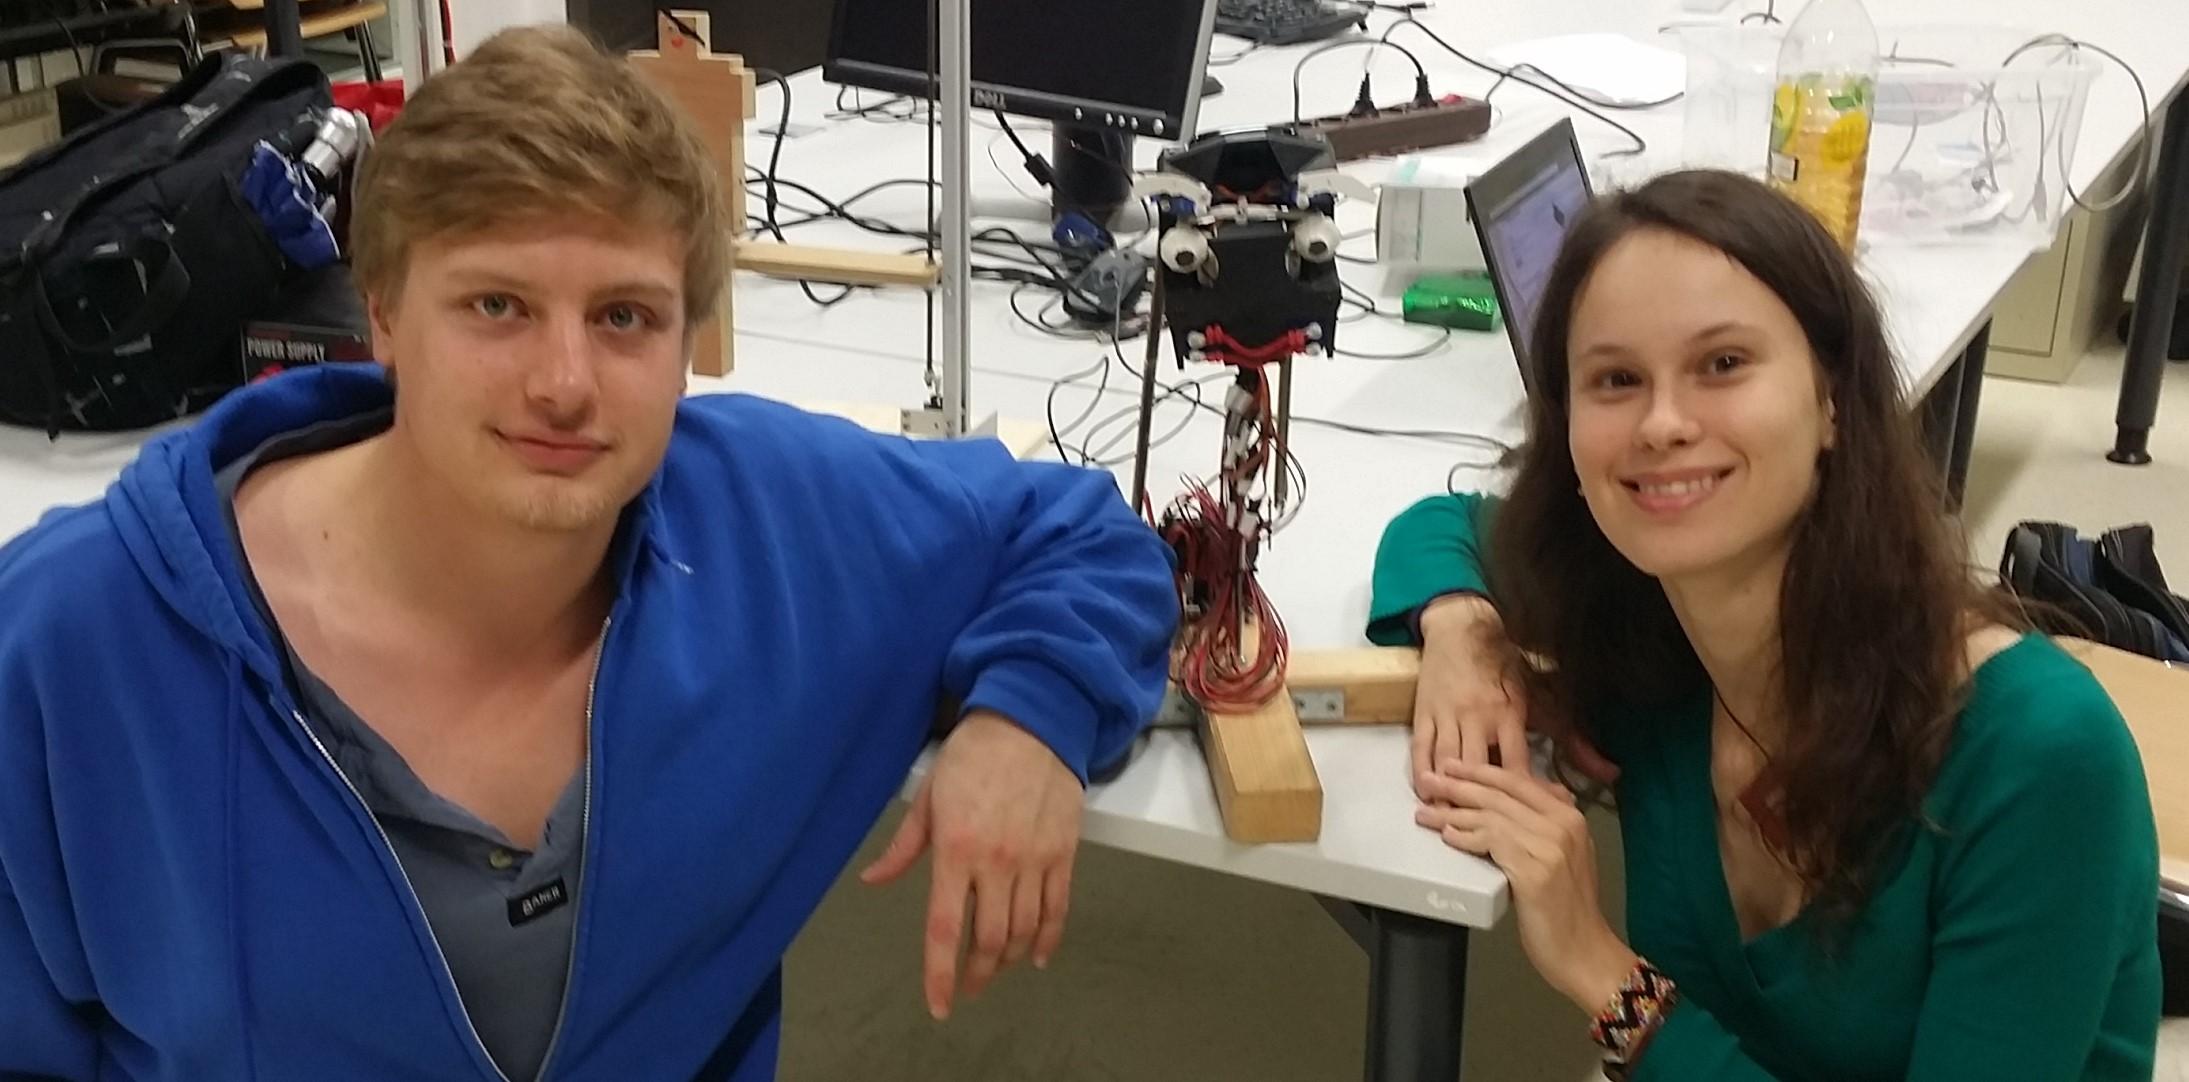
\includegraphics[width=0.88\linewidth]{images/faceEdited}
	\end{center}
	
	\section{Task:}
	The existing robotic face reacts on visual stimuli by producing acoustic and mimic signals. In order to achieve this, we implemented face and attribute recognition recognition. Furthermore, a voice output should indicate a reaction on the analysed face that RoboFace contemplates. This face is also tracked by the robot in order to maintain eye contact. 
	
	\section{Milestones:}
	\begin{itemize}
		\item overwriting the existing codebase
		\item face recognition
		\item face attribute recognition
		\item voice/sound output
		\item face tracking
	\end{itemize}

	\section{Setup guide for the robot}
	\subsection{Hardware}
	\subsection{Software}
	The elaborated C++ code for controlling RoboFace has beautiful user frienly python binaries. The following code example speaks for himself:
	>>> import face \\
	>>> f = face.Face()\\
	>>> f.sad()\\
	>>> f.happy()\\
	>>> f.unsure()\\
	>>> f.angry()\\
	>>> f.neutral()\\

	
	For using the face attribute detection software, a standard python (2.7 or 3.5) anaconda installation should additionally include \textit{opencv, keras}. You can easily install them using conda with the following commands:
	\begin{itemize}
	\item conda install -c menpo opencv3=3.1.0
	\item conda install keras
	\end{itemize}
	Then, for running the software, execute the python script \texttt{face\_detection/face\_detection.py}
	
	If you eventually want to retrain the network for further improvement of the results, then you should take a look in te \texttt{neural\_network\_training/train\_normalised.py} script.
	\subsection{Face attribute detection - the magic behind neural networks}
	\subsubsection{Architecture}
	\begin{enumerate}
		\item 	32 of neurons in each convolutional layer
		\item Activations: Relu
		\item 9 x 9 convolution $\rightarrow$ Max Pooling
		\item	7 x 7 convolution $\rightarrow$  Max Pooling
		\item	5 x 5 convolution $\rightarrow$  Max Pooling
		\item	3 x 3 convolution $\rightarrow$  Max Pooling
		\item	3 x 3 convolution $\rightarrow$  Max Pooling
		\item	Dropout(0.25)
		\item	512 Dense
		\item	Dropout(0.5)
		\item	13 Dense
		\item	Sigmoid
		\item	Binary Crossentropy
		\item	Adadelta optimiser
		\item Overall: 125,709 parameters
	\end{enumerate}
	\subsubsection{Training dataset}
	For training a neural network that generalises as much as possible, we take the big CelebA dataset, which is freely available at http://mmlab.ie.cuhk.edu.hk/projects/CelebA.html . It contains 202.599 images of 10.177 celebrities annotated with 40 attributes per image.

	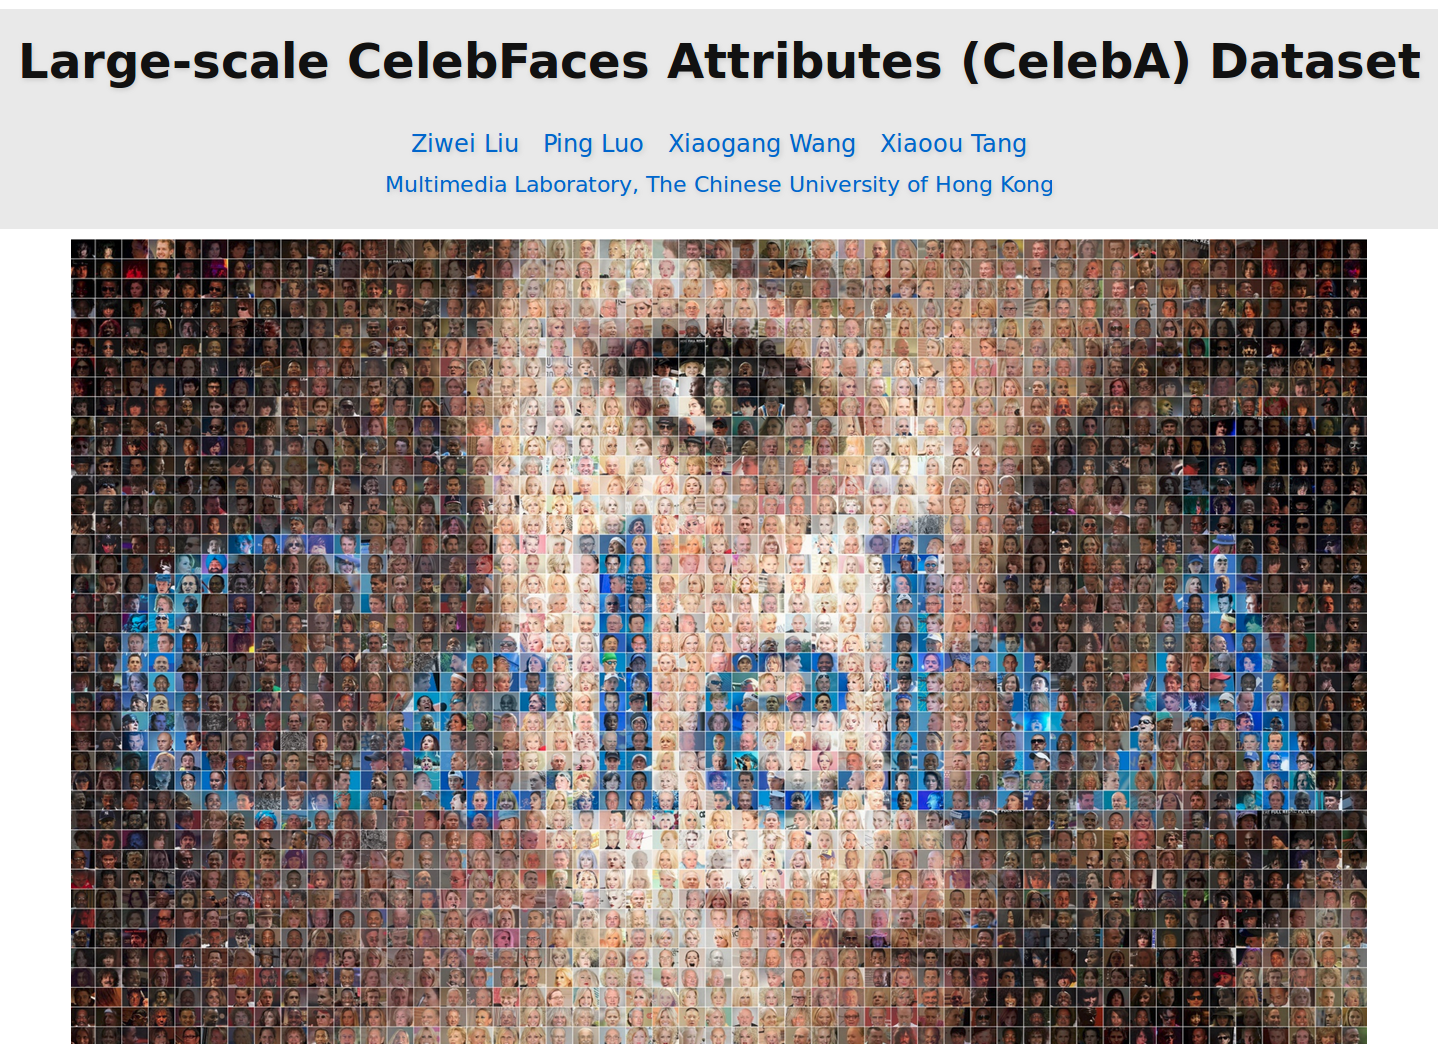
\includegraphics[width=0.5\linewidth]{images/CelebA} \\
	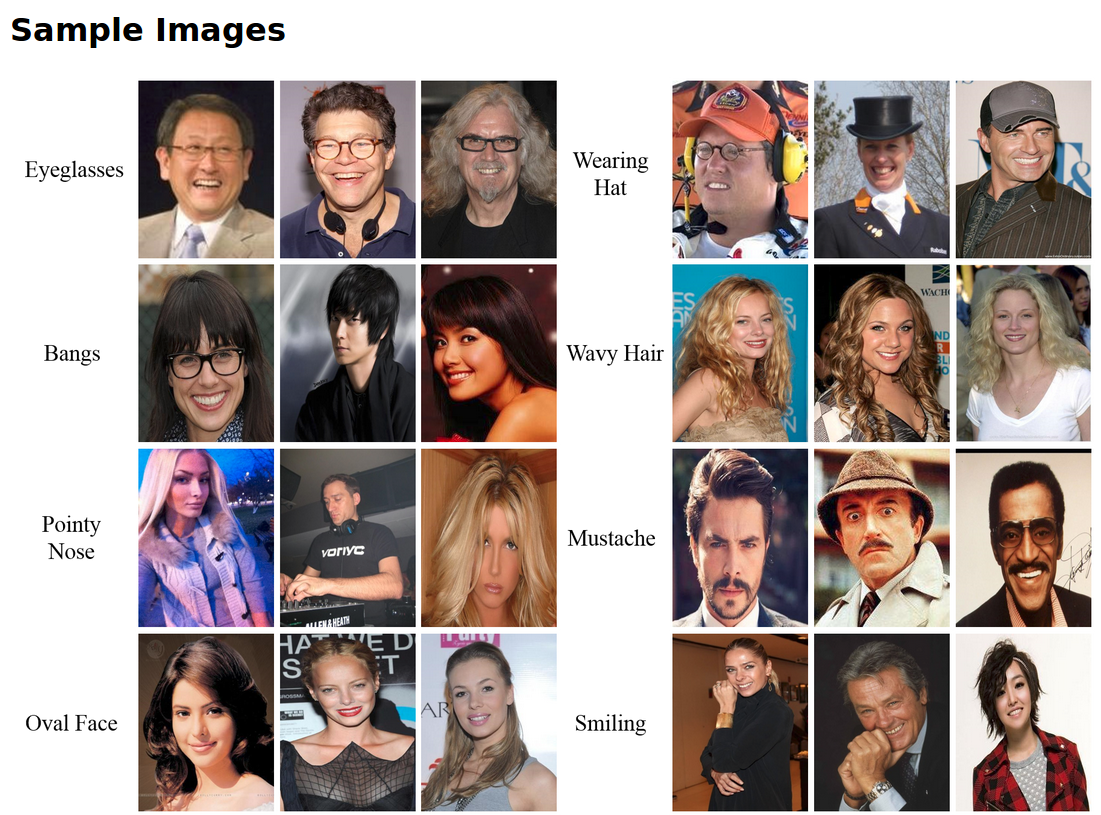
\includegraphics[width=0.5\linewidth]{images/CelebAExamples}
	
	From this attributes, we take 13 that are based only of the face region (so not taking the neck, shoulders or head top into account) and those where we think RoboFace could make something of. These are:
		\begin{enumerate}
			\item Black Hair
			\item Blond Hair
			\item Brown Hair
			\item Eyeglasses
			\item Gray Hair
			\item Male
			\item Mouth Slightly Open
			\item No Beard
			\item Smiling
			\item Straight Hair
			\item Wavy Hair
			\item Wearing Earrings
			\item Wearing Lipstick
		\end{enumerate}
	\subsubsection{Training the neural network}
	For training the neural network, we make use of the parallelizing capacity of the GPU, which results into a training time of 2 seconds per 1024 images. CPU training is obviously much slower.
	The optimiser for finding a good local optimum of the loss function is the Adadelta optimiser from keras, which stands out for his adaptive learning rate and faster convergence than normal stochastic gradient descent SGD. The overall 125.709 parameters are found in this way.
	\subsubsection{Normalising the data}
	A wrong way to train the neural network is to feed in the CelebA images from the dataset exactly as they are. Even though the training curve looks very fine, since we achieve a low loss value and a high accuracy on the training set and on the test set, the neural network over-fits the CelebA dataset and does not generalise at all on real world images as taken from RoboFace. He completely fails by saying that in the following image, there is a male with no beard with probabilities around 90\%
	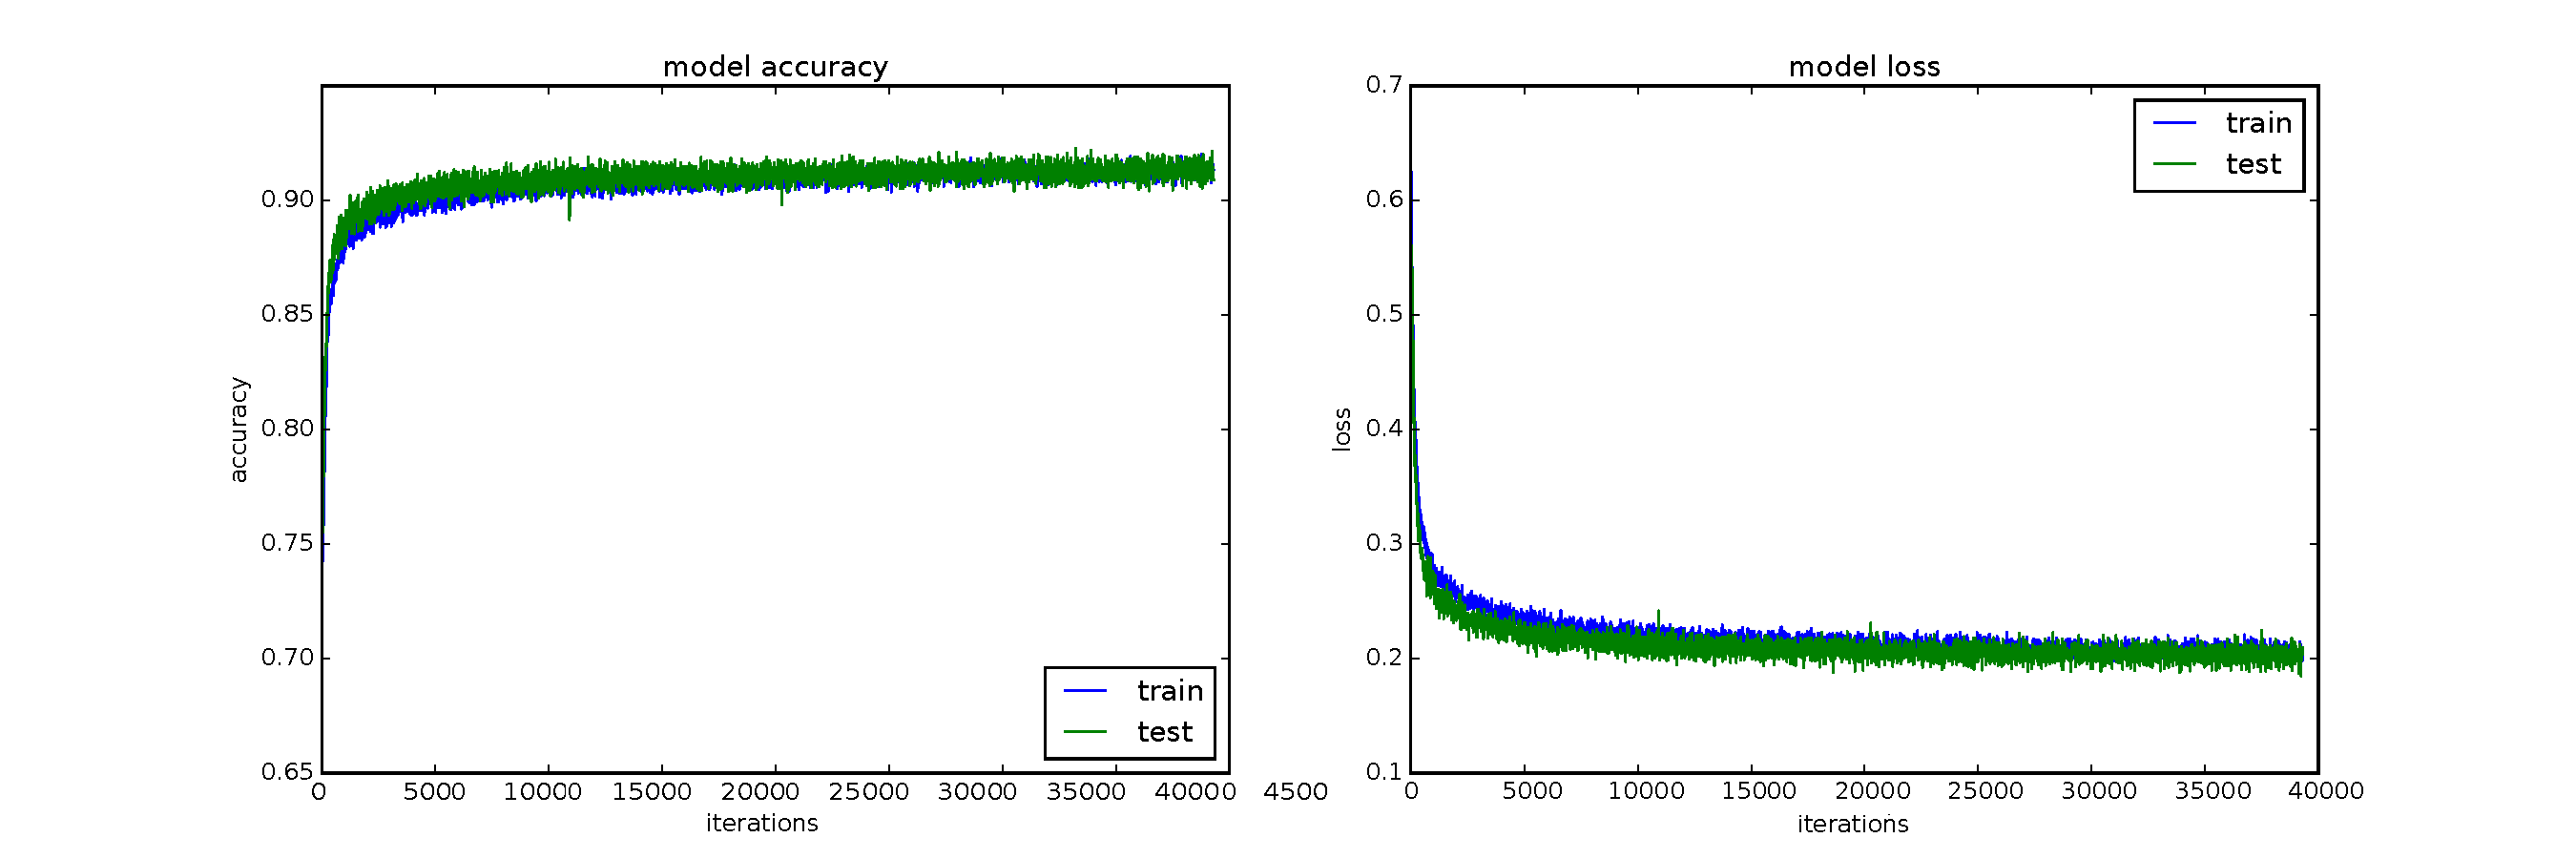
\includegraphics[width=\linewidth]{images/lossBad}\\
	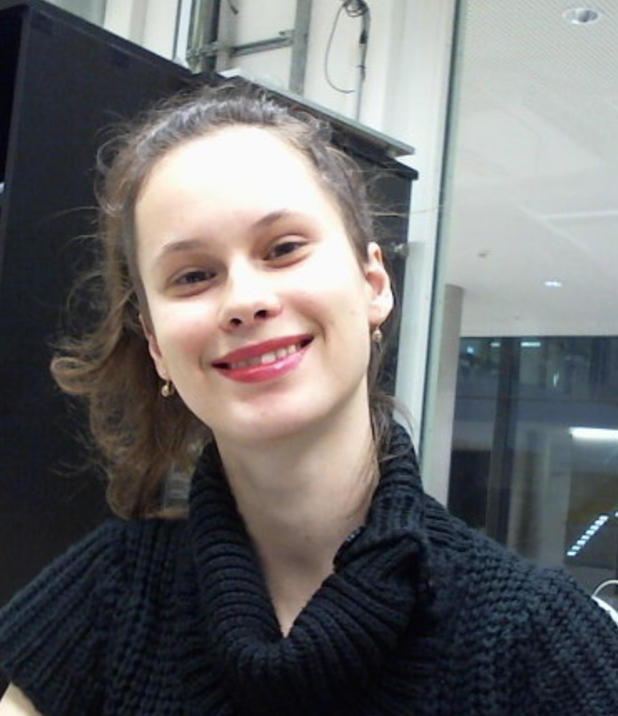
\includegraphics[width=0.2\linewidth]{images/failMaleNoBeard}\\
	
	The write way too do it, is by normalising the training and the test set, as well as the images taken by RoboFace. This is done in \texttt{neural\_network\_training/normalisation.py} the following steps:
	\begin{enumerate}
	\item center the eyes
	\item resize images to have the same inter ocular distance
	\item rotate image to make the inter ocular line look horizontal
	\item resize image to 128 x 128 pixels
	\item subtract the mean face
	\end{enumerate}

	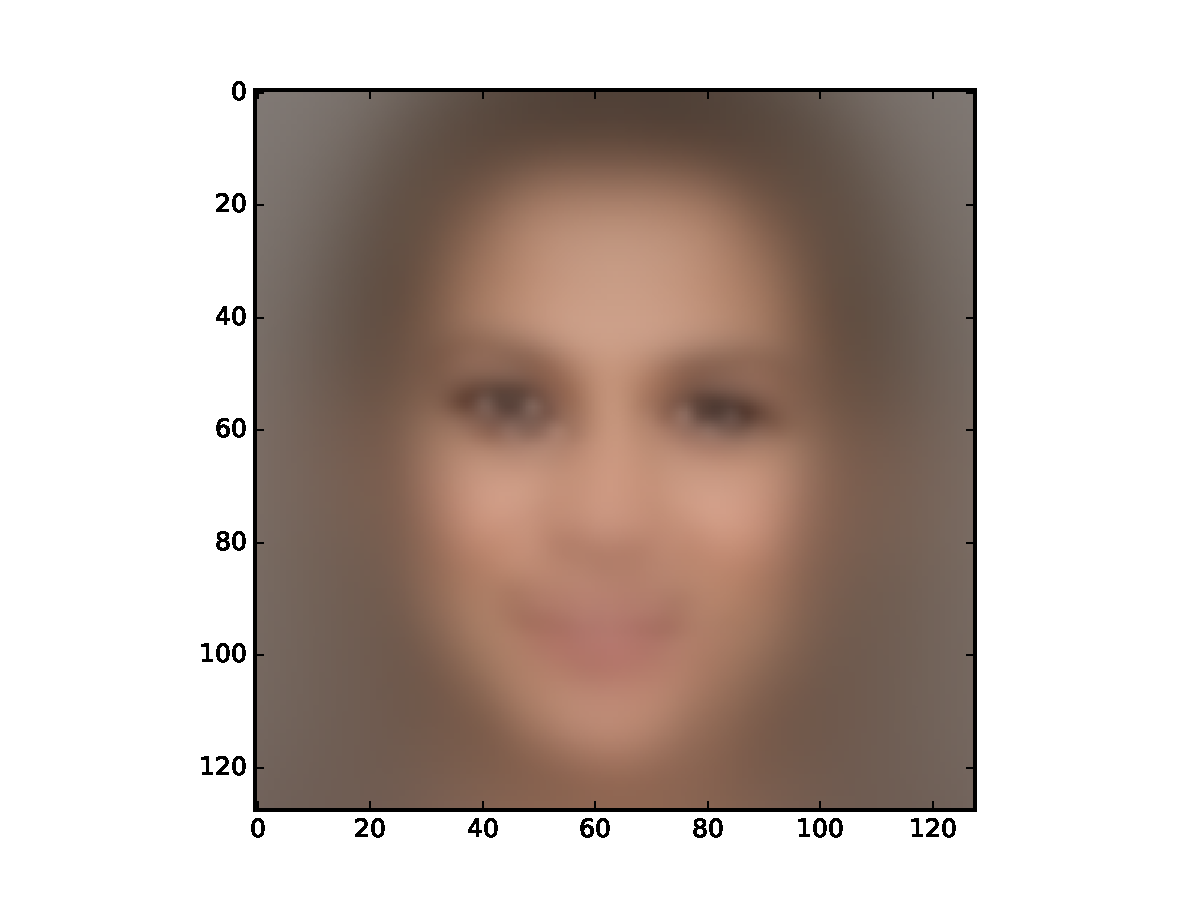
\includegraphics[width=0.5\linewidth]{images/meanFace}\\
	Now, the loss-accuracy curve looks as well as before, but the generalisation capabilities are vastly enhanced.
	
	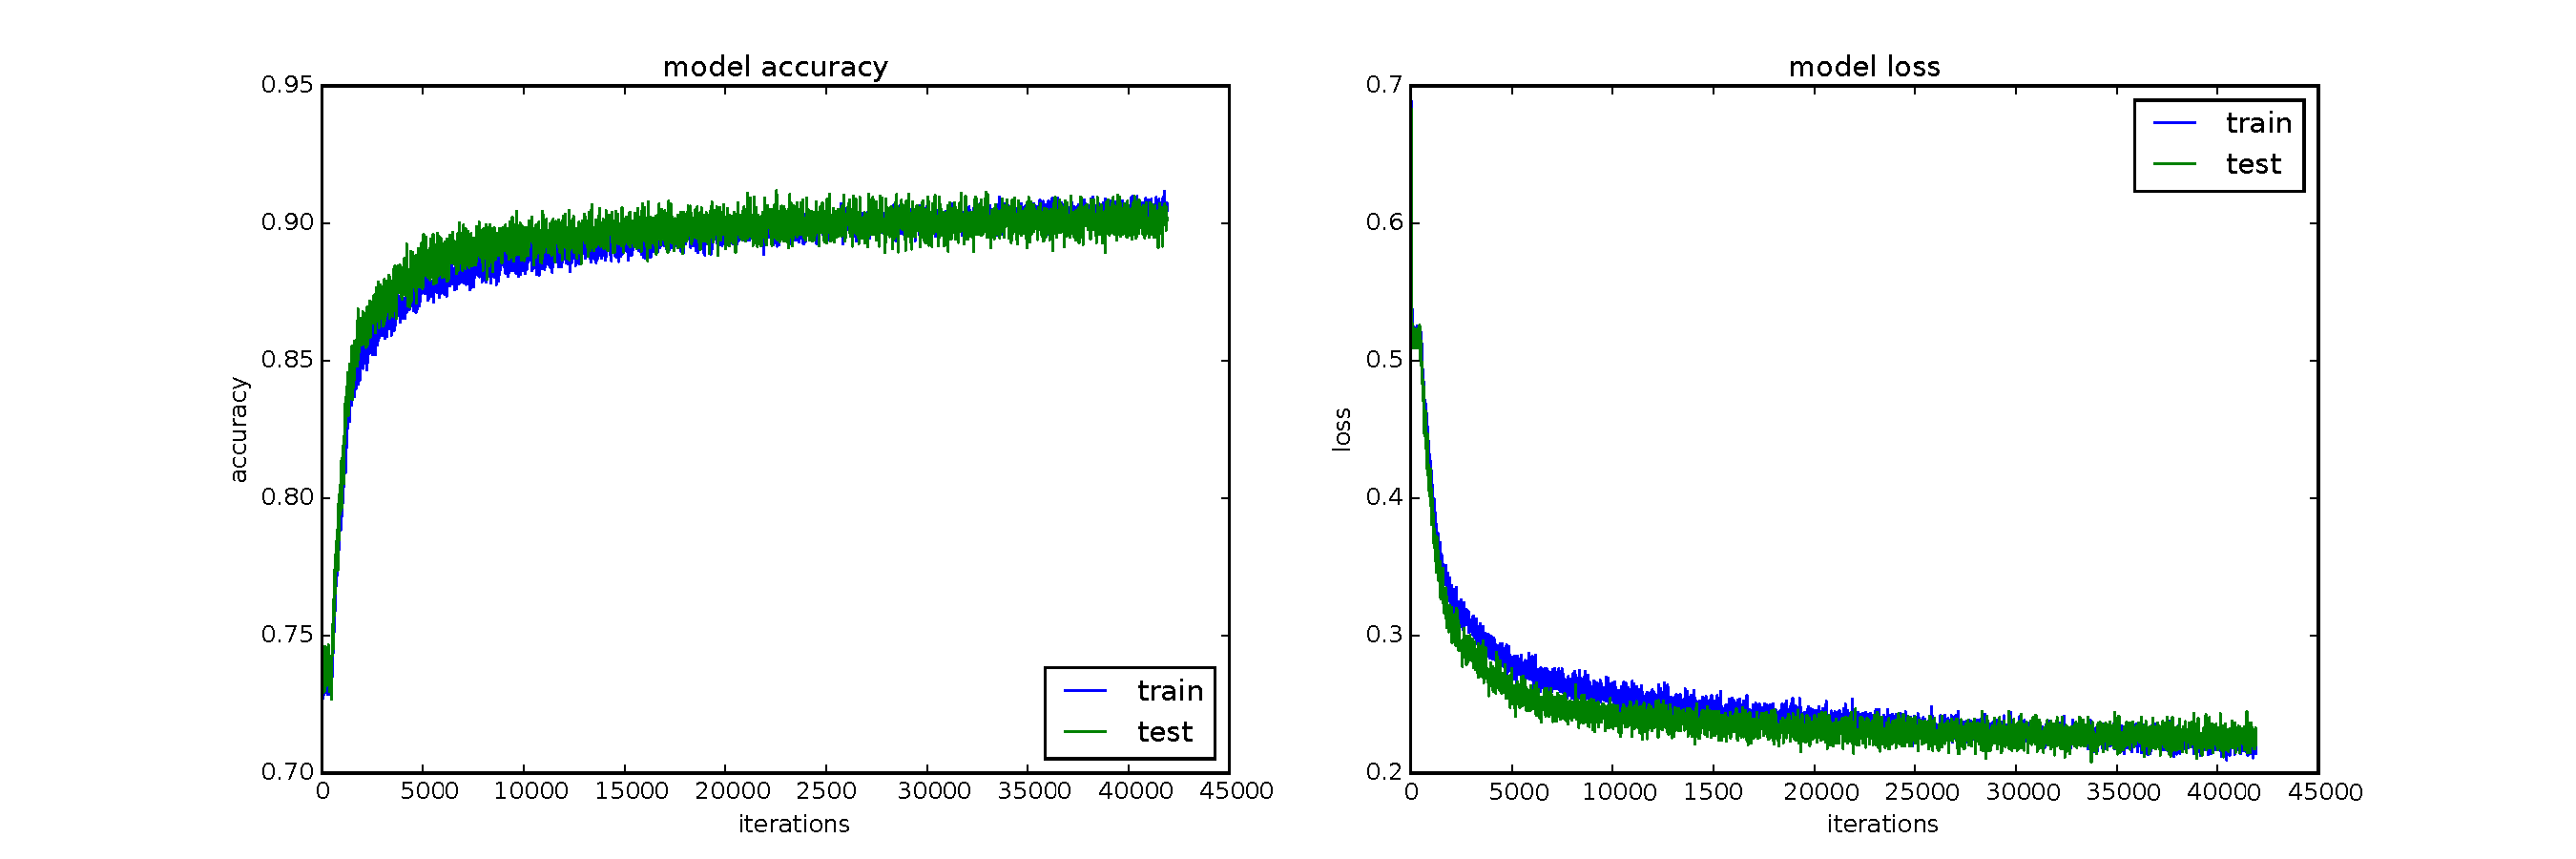
\includegraphics[width=\linewidth]{images/lossGood}\\
	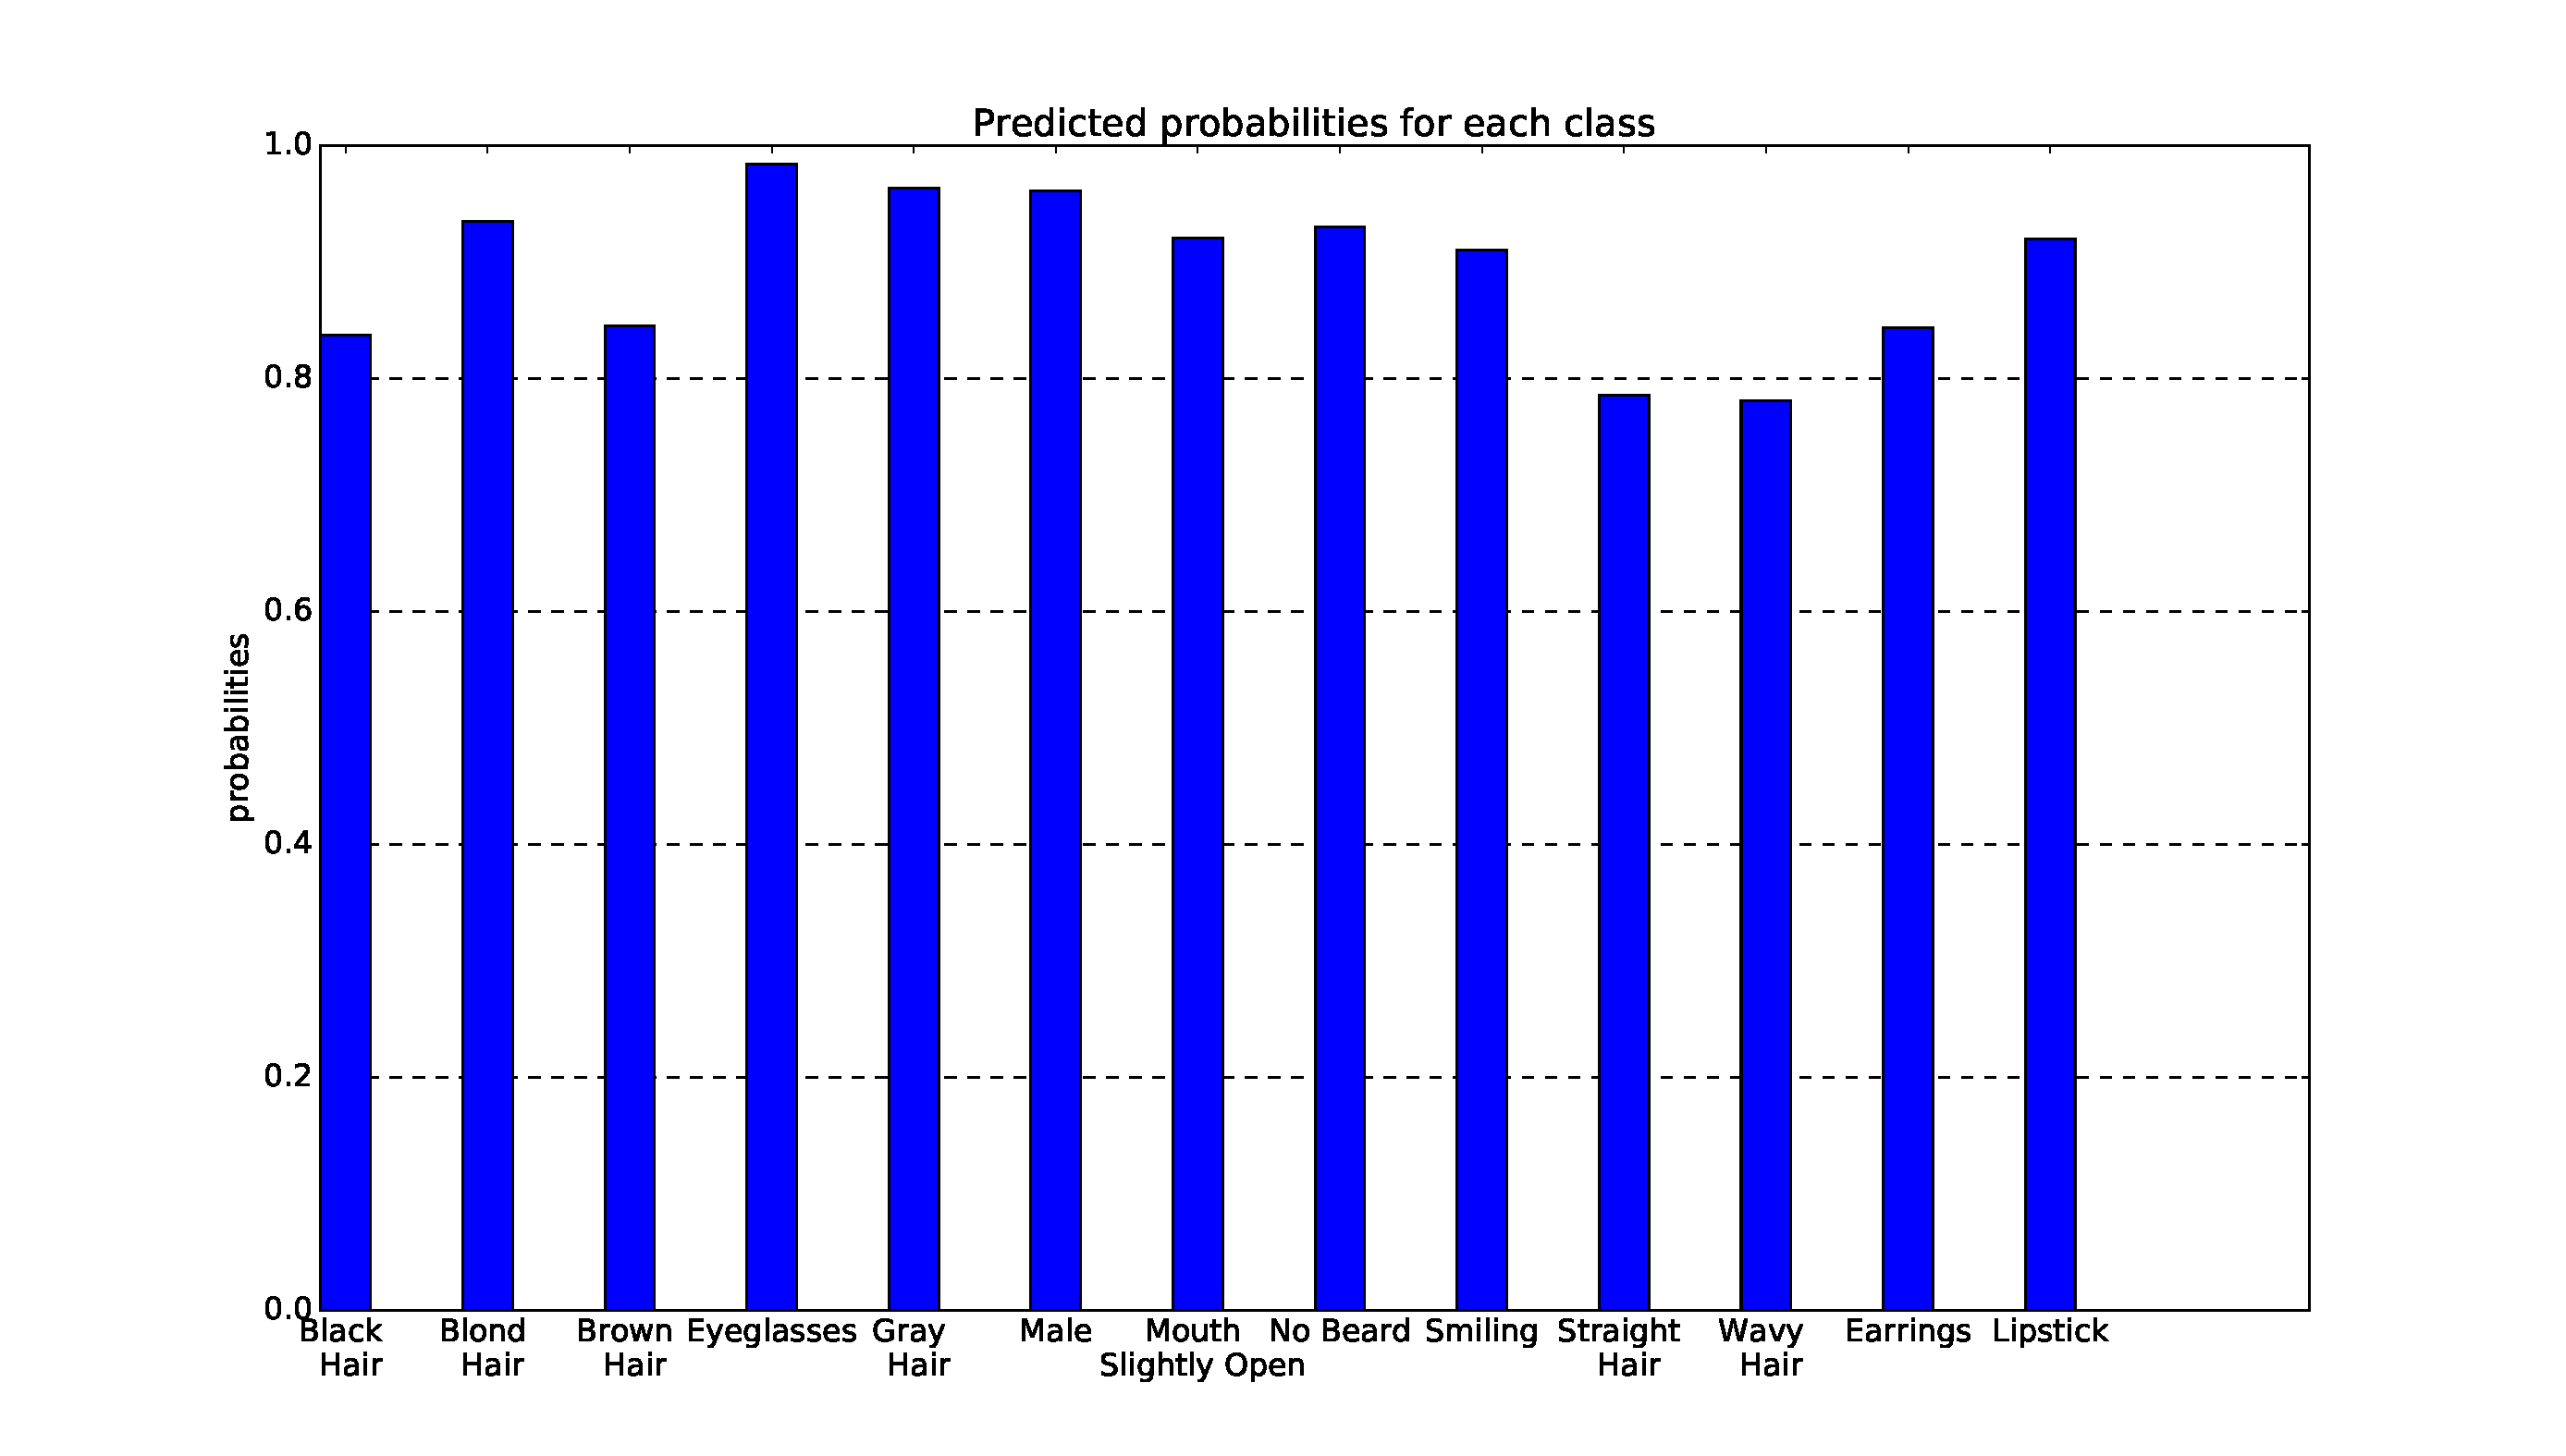
\includegraphics[width=0.8\linewidth]{images/accuracy_on_classes}
	
	'Black Hair', 'Mouth Slightly Open', 'No Beard', 'Smiling', 'Wearing Earrings', 'Wearing Lipstick' \\
	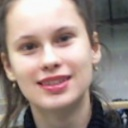
\includegraphics[height=0.1\textheight]{images/leti_normalised110} \\ 
	'Black Hair', 'Mouth Slightly Open', 'No Beard', 'Straight Hair', 'Wearing Lipstick' \\
	
\includegraphics[height=0.1\textheight]{images/leti_normalised111} 
	
	On another day, when having another look, he also performs fine:
	
	'Black Hair', 'Mouth Slightly Open', 'No Beard', 'Smiling', 'Straight Hair', 'Wearing Earrings', \emph{'Wearing Lipstick}
	 \\
	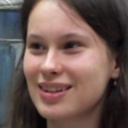
\includegraphics[height=0.1\textheight]{images/leti_normalised24}\\
	
	Indeed, the following errors are done in 2 out of 45 examples. But this small amount is no problem, since we have a continuous frame and prediction stream from the robot. If for example, he predicts the stream 'male, male, female, male, male', it is clear that we can exclude this error in a post-processing step.
	
	'Black Hair', \emph{'Male'}, 'Straight Hair'\\
	
\includegraphics[height=0.2\textheight]{images/leti_normalised0}
	\section{Outlook}
	Hardware improvements
	\section{Source code}
	Can be found on	https://github.com/LetiP/RoboFace
	
\end{document} 